\chapter{Programación}

El software de la placa ha sido desarrollado durante el transcurso de este proyecto. Se ha usado el lenguaje de programación C y el entorno de desarrollo \gls{PlatformIO} en Visual Studio Code. A continuación se detallarán los aspectos más importantes de la programación de la placa, diseños de las funciones y estructura del código, estructura general de la máquina de estados y las funciones de cada uno de los estados.

También se detallará la estructura de la memoria flash de la placa, donde se guardan los datos de configuración y los datos de la batería.

Se explicará por qué se han tomado ciertas decisiones de diseño del microcontrolador y cómo se han implementado.

\begin{tcolorbox}[colback=blue!5!white, colframe=blue!55!white, title=Nota]
    Durante la mayor parte del desarrollo se ha utilizado una placa comercial para ir programando, ya que no se tenía acceso al producto final. Ver el apéndice \ref{ApendicePruebas} para saber cómo se han realizado las pruebas del software.  
\end{tcolorbox}

\section{Plataforma}
Como se decidió en el capítulo de diseño \ref{CapDiseño} en la sección \ref{DiseñoPlatformIO}. Se ha usado \gls{PlatformIO} como entorno de desarrollo. \gls{PlatformIO} es un entorno de desarrollo que permite programar en varios lenguajes de programación y para varios microcontroladores. En este caso se ha usado para programar en C para el microcontrolador ESP32.

Para poder usar \gls{PlatformIO} vamos a necesitar instalar Visual Studio Code. Para instalar Visual Studio Code basta con ir a la página web de Visual Studio Code y descargar el instalador. Para instalar \gls{PlatformIO} basta con instalar la extensión de \gls{PlatformIO} en Visual Studio Code. Para ello basta con ir a la pestaña de extensiones en Visual Studio Code y buscar \gls{PlatformIO}. Una vez instalada la extensión de \gls{PlatformIO} ya se puede usar \gls{PlatformIO} en Visual Studio Code.

En \gls{PlatformIO} vamos a comenzar configurando el proyecto. Para que automáticamente se configure el proyecto con las librerías necesarias y el microcontrolador correcto. Para ello vamos a crear un nuevo proyecto en \gls{PlatformIO} y seleccionamos el microcontrolador ESP32.

Después vamos a crear el archivo platformio.ini en la raíz del proyecto. En este archivo vamos a configurar el microcontrolador y las librerías necesarias para el proyecto. En este caso vamos a usar las librerías de Adafruit NeoPixel, NimBLE-Arduino y TFT\_eSPI. Estas librerías se pueden instalar desde el gestor de librerías de \gls{PlatformIO}. Para ello basta con añadir las librerías al archivo platformio.ini. En este caso se han añadido las librerías en el archivo platformio.ini como se muestra en el código \ref{code:ConfiguracionPlaftformIO}.

\begin{itemize}
\item Adafruit NeoPixel
\item NimBLE-Arduino
\item TFT\_eSPI
\end{itemize}
\label{LibreriasPlatformIO}

Hay algunas recomendaciones en el uso de \gls{PlatformIO}. Para la ESP32S3, en concreto para la placa de desarrollo ESP32-S3-DevKitC-1. Se recomienda usar un filtro de monitor serie para poder ver los mensajes que envía la placa sin información adicional y que no sea relevante. Para ello se puede usar el siguiente filtro:

\begin{lstlisting}[style=console, language=bash, caption={Filtro recomendado de \gls{PlatformIO}}, label={code:FiltroEspecial}]
monitor_filters = esp32_exception_decoder
\end{lstlisting}
\newpage
El archivo de configuración platformio.ini será el descrito en el código \ref{code:ConfiguracionPlaftformIO}, donde se configura el microcontrolador, las librerías y algunas opciones de compilación y entorno. Con este fragmento el proyecto se configurará automáticamente con las librerías necesarias y el microcontrolador correcto, dejando el proyecto listo para programar. Las librerías necesarias son las descritas en la sección \ref{DiseñoLibrerias}.

\begin{lstlisting}[style=console, language=bash, caption={Configuracion \gls{PlatformIO}}, label={code:ConfiguracionPlaftformIO}]
    [env:esp32-s3-devkitc-1]
    platform = espressif32
    board = esp32-s3-devkitc-1
    framework = arduino
    board_build.f_flash = 80000000L
    board_build.flash_mode = qio
    board_build.flash_size = 16MB
    board_build.usb_cdc = 1
    upload_speed = 921600
    monitor_speed = 115200
    board_name = ModernWood
    board_upload.vid = 0x2001
    board_upload.pid = 0x1111
    lib_deps = 
        adafruit/Adafruit NeoPixel@^1.11.0
        h2zero/NimBLE-Arduino@^1.4.1
        bodmer/TFT_eSPI@^2.5.30
    build_flags =
        -I modules/include
        -I include
    build_src_filter = +<*> +<../modules/src/*>
    monitor_filters = esp32_exception_decoder
    check_skip_packages = yes
\end{lstlisting}

\begin{tcolorbox}[colback=blue!5!white, colframe=blue!55!white, title=Nota]
    Dado que para nuestro dispositivo \gls{HID} se quiere que sea algo que aparezca en el sistema como un teclado, se ha añadido a la configuración del proyecto las opciones de ``board\_name`` y los correspondientes nuevos \gls{PID} y \gls{VID}. Estos valores son necesarios para que el sistema operativo reconozca el dispositivo como un dispositivo nuevo y no como una placa de desarrollo. Más información en el apendice \ref{ApendicePIDVID}.
\end{tcolorbox}

\subsection{Compilación y entorno}

Para compilar el proyecto se puede usar el comando \textit{pio run} en la terminal de \gls{PlatformIO}. Este comando compilará el proyecto y generará el archivo binario que se puede subir a la placa. Para subir el archivo binario a la placa se puede usar el comando \textit{pio run -t upload}. Este comando subirá el archivo binario a la placa y lo ejecutará. Para ver la salida de la placa se puede usar el comando \textit{pio device monitor}. Este comando abrirá una terminal serie donde se podrá ver la salida de la placa.

También se pueden usar los botones que nos aparecen en Visual Studio Code para compilar, subir y ver la salida de la placa. Estos botones se encuentran en la parte inferior izquierda de la pantalla de Visual Studio Code. \gls{PlatformIO} por defecto detecta automáticamente el puerto serie donde está conectada la placa y la velocidad de comunicación. Si se quiere cambiar la velocidad de comunicación se puede hacer en el archivo platformio.ini en la sección de configuración del proyecto que se muestra en el código \ref{code:ConfiguracionPlaftformIO}.


\section{Interfaz}

Para la interfaz de usuario se ha usado la librería TFT\_eSPI. Esta librería es una librería de Adafruit que permite controlar pantallas \gls{TFT}. Esta librería es muy completa y permite controlar pantallas \gls{TFT} de varios tamaños y resoluciones. En este caso se ha usado una pantalla \gls{TFT} de 0.96 pulgadas y 80x160 píxeles.

Con este software se ha creado una interfaz de usuario muy sencilla. La interfaz de usuario se compone de un menú principal con 6 opciones y dentro de cada submenú hay varias opciones. La interfaz de usuario se controla con los botones del teclado. Los botones elegidos han sido Fn, Escape, las flechas de dirección y la tecla Enter. Con estos botones se puede navegar por el menú y seleccionar las opciones deseadas. Se han creado unas imágenes para cada tipo de menú y su correspondiente categoría. Estas imágenes se han guardado en la memoria flash de la placa para poder ser leídas por la pantalla \gls{TFT}. Podemos ver el menú principal en la figura \ref{fig:MenuPrincipal}.

\begin{figure}[H]
\centering
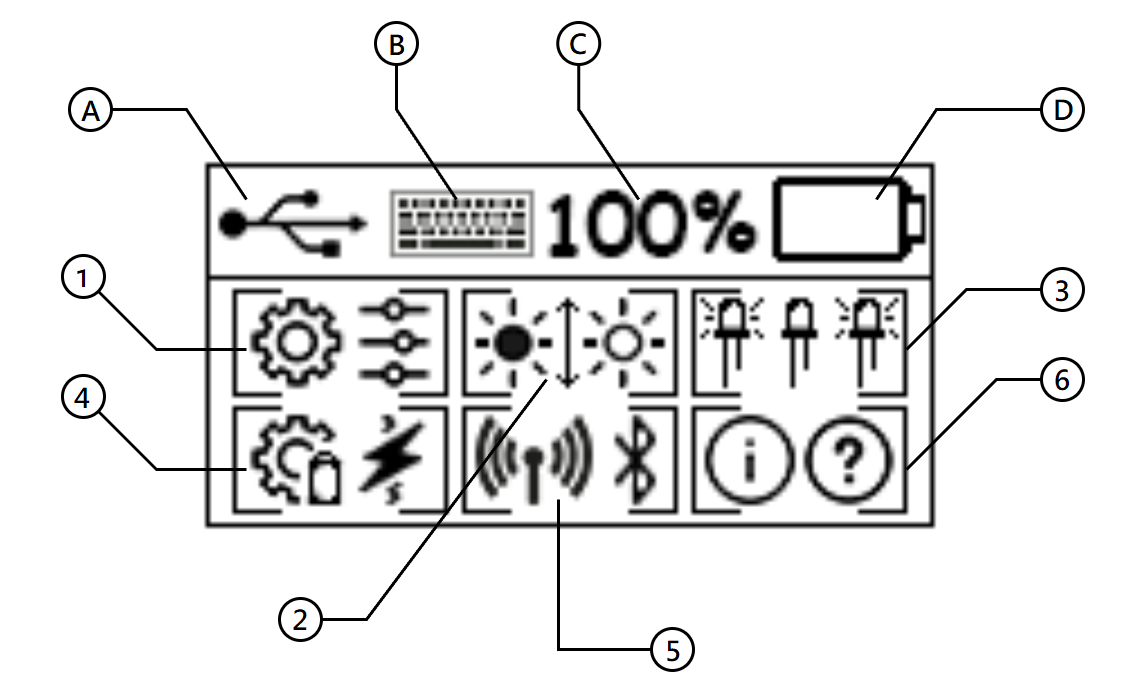
\includegraphics[width=1\textwidth]{imagenes/Capitulos/Cap07/PantallaMenuPrincipal.png}
\caption{Menú principal en la pantalla \gls{TFT} LCD 0.96``}
\label{fig:MenuPrincipal}
\end{figure}

\subsection{Menú}

El menú principal se compone de 6 opciones. Cada opción tiene un icono que corresponde a la categoría de la opción. Además, como se puede ver en la figura \ref{fig:MenuPrincipal} cada menú va a tener asociado un número. Este número es el número de la opción en el menú. Este número se va a usar para seleccionar la opción deseada. Para seleccionar una opción se va a usar la tecla Enter. Para moverse por el menú se van a usar las flechas de dirección. Para salir de una opción se va a usar la tecla Escape. Para volver al menú principal se va a usar la tecla ESC. Si se quiere entrar y salir del modo de configuración se va a usar la tecla Fn.

Los diferentes menús vienen señalados en la imagen por un número. Con este vamos a identificar al menú para poder explicar su funcionamiento. Los menús son los siguientes:
\begin{itemize}
\item 1. Ajustes
\item 2. Brillo
\item 3. Leds
\item 4. Batería y Energía
\item 5. Conexión
\item 6. Extra y Ayuda
\end{itemize}

\subsubsection{Ajustes}
Este menú se compone de varias opciones. En este menú se pueden ajustar los parámetros del funcionamiento del teclado. En este menú se pueden ajustar los parámetros de, activar y desactivar la pantalla, activar y desactivar el teclado, ajustar el tiempo de debounce del teclado y ajustar el idioma de la interfaz.

\subsubsection{Brillo}
Este menú se compone de los parámetros de brillo de la pantalla y de los \glsnocase{LED}s. En este submenú se pueden encontrar dos ajustes numéricos del 0 al 100. Estos ajustes son el brillo de la pantalla y el brillo de los \glsnocase{LED}s. También se pueden llegar a apagar los \glsnocase{LED}s y la pantalla mediante este submenú, ya que podemos poner el brillo a 0.

\subsubsection{\gls{LED}s}
Este menú se compone de los parámetros de los \glsnocase{LED}s. En este submenú se pueden encontrar los ajustes de activar o desactivar los \glsnocase{LED}s, el color de los \glsnocase{LED}s y el modo de los \glsnocase{LED}s y la velocidad de los \glsnocase{LED}s.

\subsubsection{Batería y Energía}
Este menú se compone de los parámetros de la batería y la energía. En este submenú se pueden encontrar los ajustes de la batería. Para este submenú encontramos activar o desactivar la batería y activar o desactivar el modo de ahorro de energía.

\subsubsection{Conexión}
Este menú se compone de los parámetros de la conexión. En este submenú se pueden encontrar los ajustes de la conexión. Podemos seleccionar activar el modo de \gls{Bluetooth} por preferencia, activar o desactivar el \gls{Bluetooth} y seleccionar como preferente el modo \gls{USB} sobre el modo \gls{Bluetooth}.

\subsubsection{Extra y Ayuda}
Este menú se compone de los parámetros de la ayuda y extras. En este submenú encontramos el restaurar la configuración de fábrica, el modo especial para las funciones programas por el usuario y dos opciones de información y ayuda.

\subsection{Barra de estado}

La barra de estado se compone de varios elementos. En la parte superior de la pantalla se puede ver el icono de la conexión (A), el icono del modo de funcionamiento del teclado (B), el porcentaje de batería restante (C) y el icono de la batería (D). Estos elementos se pueden ver en la figura \ref{fig:MenuPrincipal}.

\begin{itemize}
    \item \textbf{A}. Icono de la conexión: Este icono indica el estado de la conexión. Este puede alternar entre el icono de \gls{Bluetooth} y el icono de \gls{USB}.
    \item \textbf{B}. Icono del modo de funcionamiento del teclado: Este icono indica el estado del teclado. Este puede alternar entre el icono de teclado activado y el icono de configuración.
    \item \textbf{C}. Porcentaje de batería restante: Este porcentaje indica el porcentaje de batería restante que se actualiza cada 1 minuto.
    \item \textbf{D}. Icono de la batería: Este icono indica el estado de la batería. Este indica si la batería está cargando o si la batería está descargada. También indica la carga y posee colores para indicar el estado de la batería.
\end{itemize}

\section{Funcionalidad}

La funcionalidad de la placa se ha dividido en varios apartados. Cada apartado se ha dividido en varios estados. Cada estado se compone de varias funciones que se ejecutan en función del estado en el que se encuentre la placa. Para cambiar de un estado a otro se han usado variables de estado a lo largo del código. Estas variables nos indican en que modo estamos, en que menú estamos, en que opción estamos, si hemos cambiado alguna opción, si hemos pulsado algún botón, etc.

Lo que nos permite desde el bucle principal saber en qué estado nos encontramos de la ejecución del programa y que funciones debemos ejecutar en cada momento. A continuación se detallarán los diferentes estados de la placa y las funciones que se ejecutan en cada uno de los estados.

\subsection{Estados}
\subsubsection{Ahorro de energía}
El primer apartado es el ahorro de energía. En esta sección de código se comprueba si el flag de tiempo de ahorro de energía ha sido activado por interrupción hardware de un reloj. Si el flag está activado, se activa el modo de ahorro de energía y se desactiva la pantalla y los \glsnocase{LED}s. Si el flag está desactivado y el flag de que estamos durmiendo está activado, se despierta la pantalla y los \glsnocase{LED}s.

\subsubsection{Batería}
Aquí comprobamos si desde el gestor de interrupciones de la batería ha actualizado el valor de la misma. Si el valor ha variado, se actualiza el valor de la batería en la pantalla y se actualiza el icono de la batería.

\subsubsection{\gls{LED}s}
En esta sección se comprueba si los \glsnocase{LED}s están activados en la configuración y si el modo de los \glsnocase{LED}s es el modo de \glsnocase{LED}s programados por el usuario. Si es así se ejecuta el modo de \glsnocase{LED}s programados por el usuario. Si no se ejecuta el modo de \glsnocase{LED}s por defecto.

\subsubsection{Actualización de conexión}
En esta sección se comprueba si la conexión ha cambiado. Si ha cambiado, se actualiza el icono de la conexión y se actualiza el modo de conexión.

\subsubsection{Pantalla}
En esta sección se comprueba si la pantalla está activada. En el caso de estar activada, se comprueba que se ha cambiado el estado de la pantalla. En el caso afirmativo se actualiza la pantalla con la información necesaria, además, de mostrar siempre la pantalla con el brillo seleccionado.

\subsubsection{Teclado}
Se comprueba primero que no estamos en el modo de teclas especiales o modo especial, ya que tendríamos que ejecutar la función especificada especial.
Si no estamos en el modo especial se procede a funcionar en modo normal del teclado, mientras se comprueba que el flag de la interrupción de la tecla Fn no este activado. Si está activado, se cambia el modo de teclado a configuración y se activa el flag de configuración.
En el modo configuración nos encontramos con lo mismo, se comprueba que el flag de la interrupción de la tecla Fn no este activado. Si está activado se cambia el modo de teclado a normal y se desactiva el flag de configuración.

En el modo de configuración, cada vez que se pulsa una tecla se actualiza el valor de la tecla pulsada y se activa el flag de tecla pulsada, activando la función de actualizar la pantalla.

Estos estados se pueden ver en la figura \ref{fig:EstadosKeyboard} junto con la figura del diagrama de flujo del bucle principal \ref{fig:MainLoop}.

\begin{figure}[H]
    \centering
    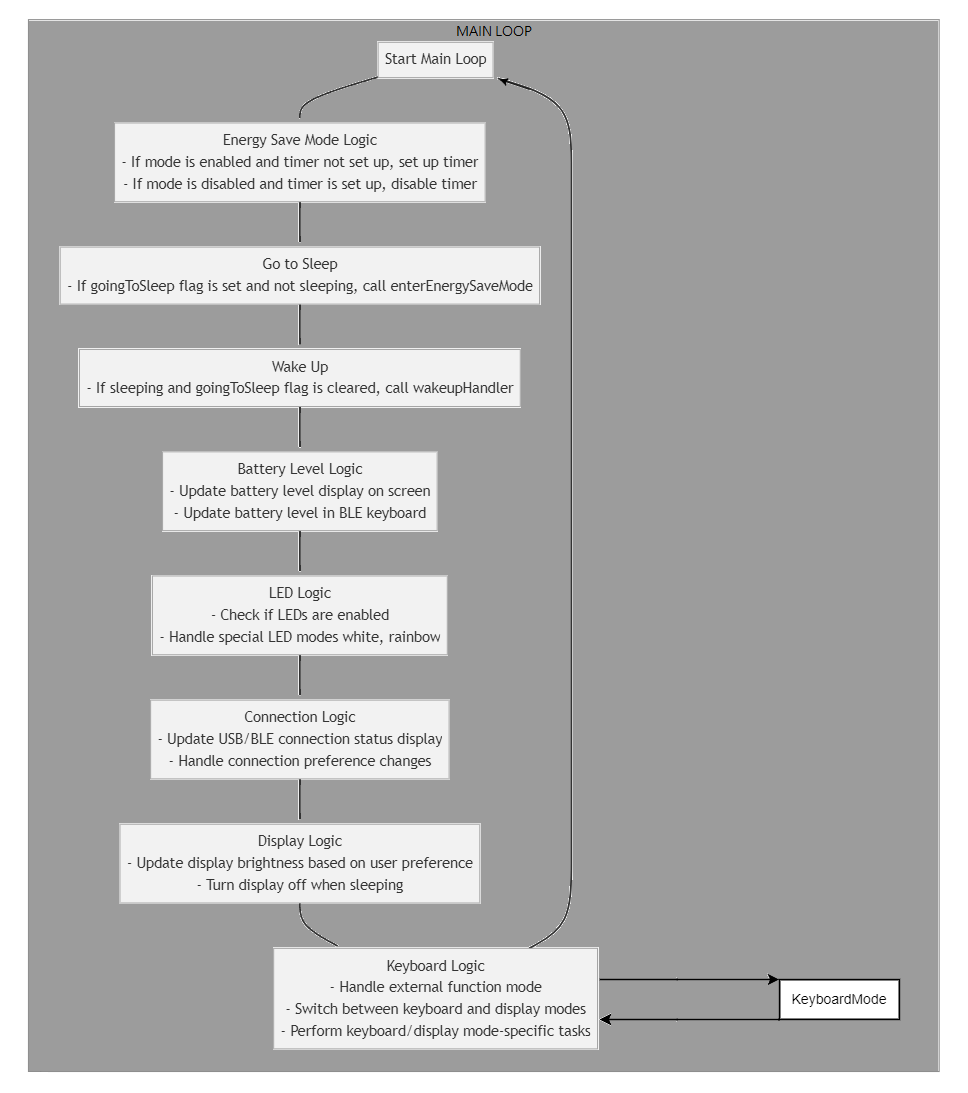
\includegraphics[width=1\textwidth]{imagenes/Capitulos/Cap07/MainLoop.png}
    \caption{Diagrama de Flujo del bucle principal}
    \label{fig:MainLoop}
\end{figure}

\begin{figure}[H]
    \centering
    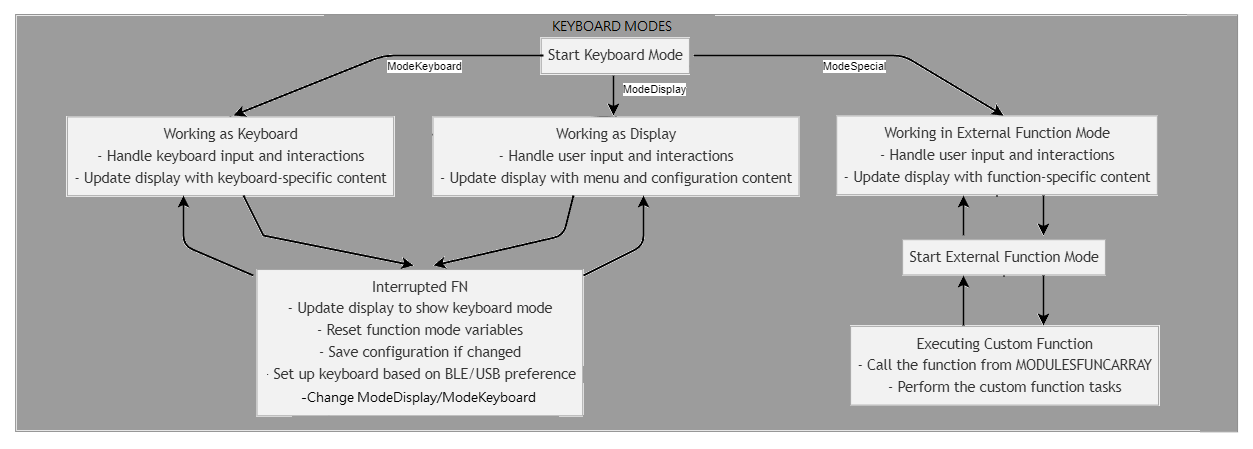
\includegraphics[width=1\textwidth]{imagenes/Capitulos/Cap07/EstadosKeyboard.png}
    \caption{Diagrama de Flujo de la secuencia de cambio de modo de teclado}
    \label{fig:EstadosKeyboard}
\end{figure}

\subsection{Conectividad}

Para la conectividad se ha decidido que sea independiente el modo \gls{Bluetooth} y el modo \gls{USB}. Para ello se ha creado un menú de configuración donde se puede seleccionar el modo de conexión preferente. Si se selecciona el modo \gls{USB} preferente, la placa se conectará por \gls{USB} siempre que esté conectado. Si se selecciona el modo \gls{Bluetooth} preferente, la placa se conectará por \gls{Bluetooth} siempre que esté conectado. Si no se selecciona ninguno de los dos modos, el teclado permanecerá desconectado. Se puede conectar por \gls{USB} y \gls{Bluetooth} a la vez, pero en tal caso tendrá preferencia el modo \gls{USB}.

\subsection{Leds}

Para los \glsnocase{LED}s se han creado varios modos de funcionamiento. Se ha creado el modo estático, donde el color seleccionado se mantiene fijo. El modo de color blanco y el modo arcoíris. Se podrán añadir más modos creando la función correspondiente y añadiéndola al menú de \glsnocase{LED}s. Revisar el apéndice \ref{ApendiceLeds} para más información.

\subsection{Macros}

Para los macros o funciones especiales, se tendrá que activar el modo desde el menú ``Extra y ayuda'', ya que estas funciones serán creadas por el usuario y se tendran que añadir al código. Se podrán añadir más funciones creando la función correspondiente y añadiéndola al menú de macros. Revisar el apéndice \ref{ApendiceMacros} para más información.

\section{Boot}

Para poder cargar el código al microcontrolador se ha usado el conversor \gls{TTL} que se indicó en la sección \ref{DiseñoActualizaciones} se ha usado un conversor de nivel lógico para poder programar el chip mientras este se alimenta con el \gls{USB} 5.0 V y no con la batería.
El código una vez cargado en el microcontrolador se ejecutará en cuanto el chip revisa el voltaje necesario para funcionar. En este caso el chip se enciende en cuanto se conecta el \gls{USB} y se enciende la pantalla mostrando el logotipo del proyecto. Acto seguido se encienden los leds y se muestra el menú principal en el caso de estar activa la pantalla.

\begin{tcolorbox}[colback=red!11!white, colframe=red!50!white, title=Errores]
    Ver apartado de errores \ref{CorrienteInversa} y \ref{VoltajeRegulador} donde se explica por qué es necesario el conversor de nivel lógico.
\end{tcolorbox}